\pagebreak

\begin{center}
	{\Large \bf Facilities and Equipments}\\
%     \vspace{4pt}
% 	\renewcommand{\baselinestretch}{1}
%    	{\large PI: Zhi Li (Worcester Polytechnic Institute)\\
%     Co-PI: Brian Ziebart (University of Illinois at Chicago), Jie Fu (Worcester Polytechnic Institute)}
   	% \vspace{4pt}
    % {\large Worcester Polytechnic Institute}
\end{center}

\vspace{0.5em}
%-------------------------------------------------------------------------
\section{Laboratories}\label{sec:Lab}
%-------------------------------------------------------------------------

PIs Li and Fu equally share a 1500 square foot lab space with another junior faculty member at WPI. This lab space is located at 85 Prescott 224, Robotics Engineering Program, Worcester Polytechnic Institute. A motion capture system has been installed in this lab to cover a 21ft by 17ft space. The rest of the lab space is sufficient for performing experimental study on humans and robots, in addition to accommodating PhD students.

PI Ziebart directs the Purposeful Prediction laboratory in the Computer Science department at the University of Illinois at Chicago (UIC). This laboratory can house 20 students and is shared with Prof. Milos Zefran, Electrical and Computer Engineering, UIC. The research focus of the lab is on the development and application of
prediction techniques for application-specific performance measures. Current application areas include robotics, human-computer interaction, and wild animal behavior and activity prediction.




% PM: Would it be useful to mention additional WPI computing resources and PI work laptops, since one desktop and one laptop seems a bit small for the number of people (2 professors + graduate students) working at WPI)?

%-------------------------------------------------------------------------
\section{Major Equipments}\label{sec:equip}
%-------------------------------------------------------------------------


\begin{figure}[h!]
\mbox{
  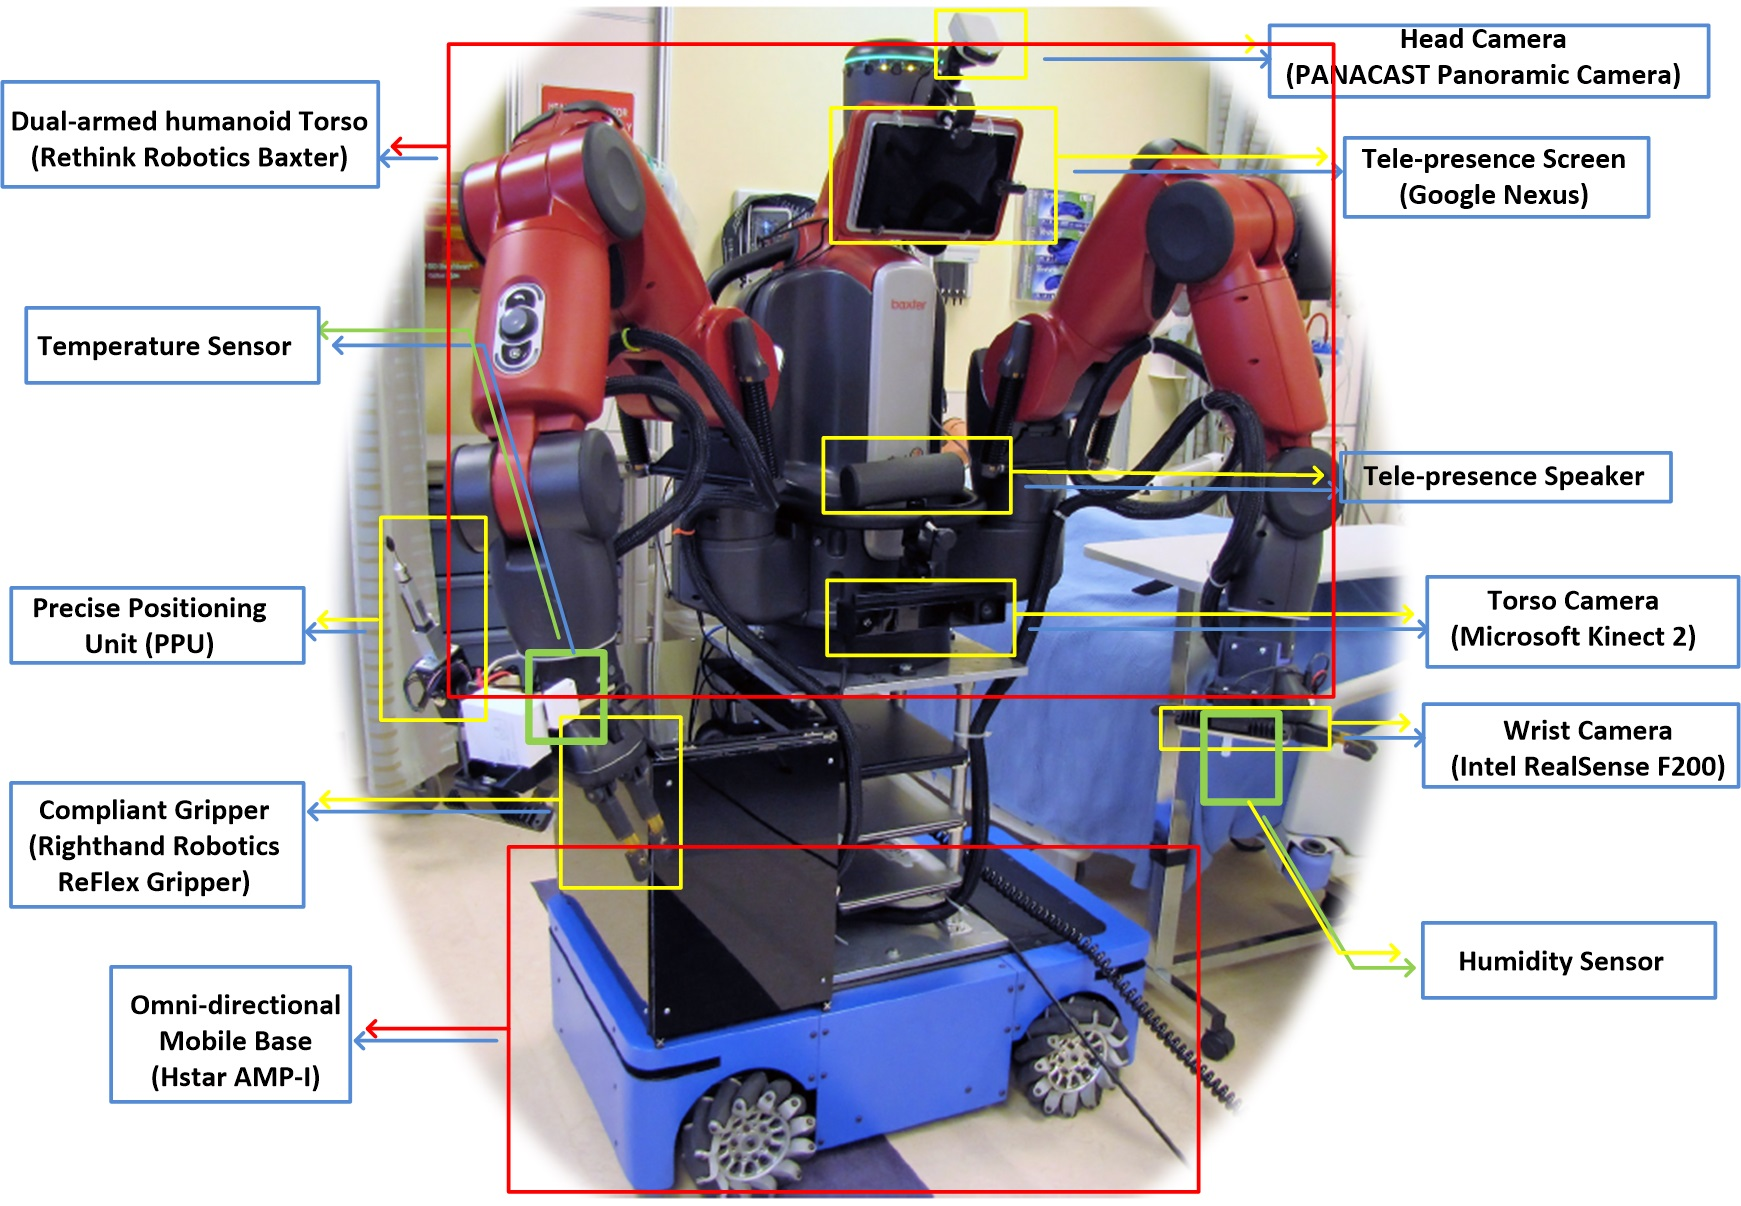
\includegraphics[width=0.48\linewidth]{fig//TRINA_Hardware_Notes}
    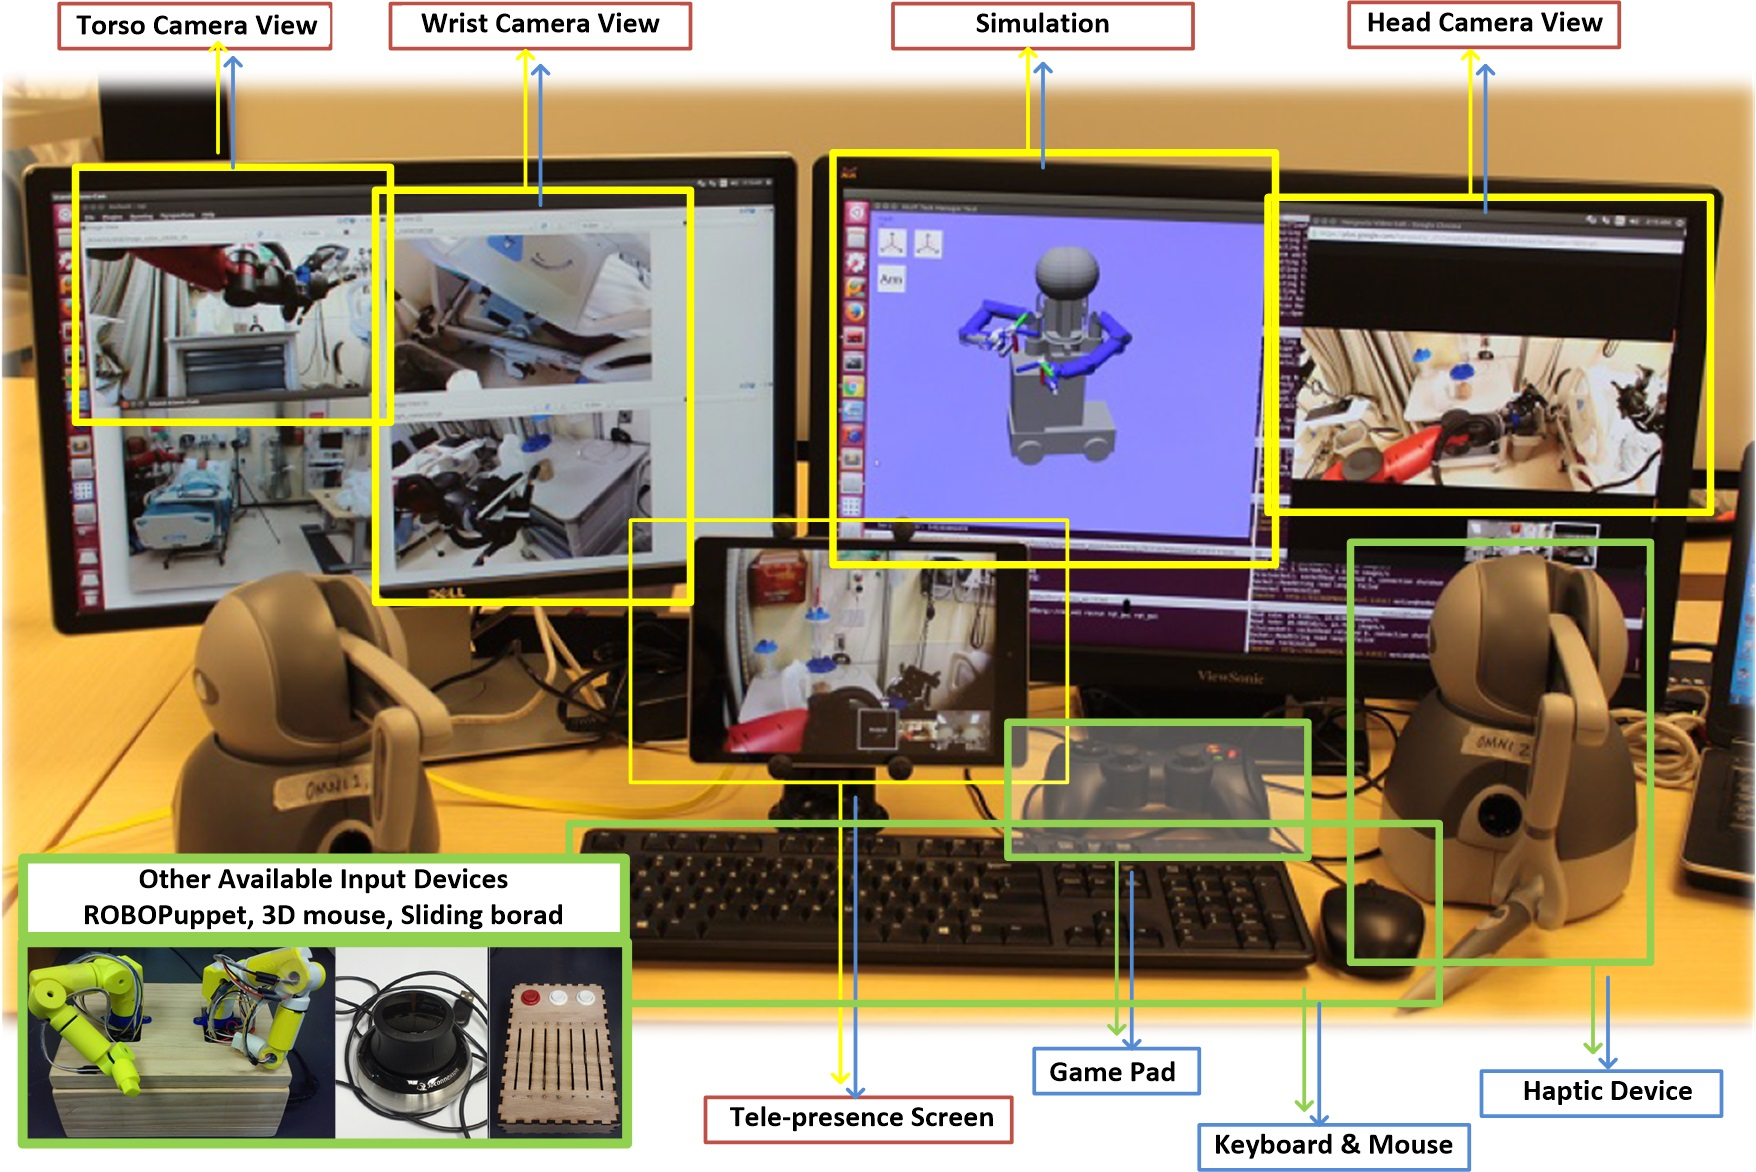
\includegraphics[width=0.48\linewidth]{fig//TRINA_Console_Notes}
}
    \caption{(Left) The Tele-robotic Intelligent Nursing Assistant (TRINA) system and (Right) its operator console which can support various modalities for direction teleoperation and shared-autonomous control.}
    \label{fig:Trina_facility}
\vspace{2ex}
\end{figure}

PI Li has a fully integrated Tele-robotic Intelligent Nursing Assistant (TRINA) system (see~\fig{fig:Trina_facility}). A Da Vinci surgical robot console is also available as an additional robot teaching interface. PIs Li and Fu share a Vicon motion capture system, with 10 Vicon Vero 2.2 cameras. PI Ziebart has a Rethink Robotics Baxter platform, Microsoft Kinect 3D cameras and an HTC Vive virtual reality system.

%-------------------------------------------------------------------------
\section{Computing Resources}\label{sec:Computers}
%-------------------------------------------------------------------------

\paragraph*{Computers} Li and Fu's lab has two desktop and one laptop computers dedicated for students work on this project. PI Ziebart has one workstation equipped with graphical processor units for running real-time robotics experiments, multiple servers for off-line machine learning tasks, and laptops for research assistant usage. In addition, WPI provides extensive computational resources including high speed networking, data hosting and storage and high-performance computing. Multiple platforms are available for unit testing software under different operating systems and hardware configurations. These shared computing resources can support intensive computing tasks as well as securely host data and project code. 

\paragraph*{Computer Software} 
Software for mechanical design and manufacturing, circuit board modeling and design, mathematical modeling, and software development are readily available. Workstations are available with all required programming, simulation, and modeling software and hardware. This resources can support robot platform maintenance, and develop robot accessories and experimental setups needed for system evaluation.  

%-------------------------------------------------------------------------
\section{Facility for user study and system evaluation}\label{sec:PracticePoint}
%-------------------------------------------------------------------------
The user study for system evaluation will be performed in the simulated patient room at the WPI PracticePoint. PracticePoint is a membership-based R\&D and commercialization alliance that seeks to improve healthcare technologies and develop new medical cyber-physical systems. PracticePoint will provide an agile and scalable, collaborative research facility empowering public and private universities, research institutions, industry and innovators to incorporate cyber-physical systems into medical devices and equipment that will improve performance, security, accuracy, timeliness, costs and outcomes in human healthcare. PracticePoint will foster professional collaborations among its members and partner institutions through four state-of-the-art test beds, secured project pods, collaboration suites and shared tool bays.

At the facility, members will have access to point-of-practice environments including: medical imaging coupled with a hybrid operating room suite (including an MRI scanner), a controlled care environment (reconfigurable as ICU, exam room, and recovery room), rehabilitative care suites (including motion capture and rehab equipment), and a residential setting (highly instrumented mock home environment). These point of practice care suites will be integrated with advanced manufacturing and testing equipment. It has advanced manufacturing (including CNC machining, 3D printing, laser cutting), electronics assembly and test equipment, and build areas. It will also comprise office spaces for faculty and graduate students, individual research group lab spaces, and reconfigurable “lab pods” that can be assigned to collaborating organizations or used on a short-term per-project basis. 

